\documentclass[journal,10pt]{IEEEtran}

\usepackage{amsmath,amssymb,amsthm,mathtools}
\usepackage{bm}
\usepackage{booktabs}
\usepackage{cite}
\usepackage{enumitem}
\usepackage{graphicx}
\usepackage{microtype}
\usepackage{tabularx}
\usepackage{xurl}
\usepackage[hidelinks]{hyperref}
\hypersetup{
  pdftitle={Exact Robust Local Graph-Smoother Design Under Hidden-Topology Completions},
  pdfauthor={Che Lin}
}

\newtheorem{theorem}{Theorem}
\newtheorem{corollary}[theorem]{Corollary}
\theoremstyle{definition}
\newtheorem{definition}[theorem]{Definition}
\newtheorem{example}[theorem]{Example}
\theoremstyle{remark}
\newtheorem{remark}[theorem]{Remark}

\newcommand{\R}{\mathbb R}
\newcommand{\Sph}{\mathbb S}
\newcommand{\one}{\mathbf 1}
\newcommand{\conv}{\operatorname{conv}}
\newcommand{\cl}{\operatorname{cl}}
\newcommand{\diag}{\operatorname{diag}}
\newcommand{\tr}{\operatorname{tr}}
\newcommand{\dist}{\operatorname{dist}}
\newcommand{\supp}{\operatorname{supp}}
\newcommand{\rank}{\operatorname{rank}}
\newcommand{\cX}{\mathcal X}
\newcommand{\cP}{\mathcal P}
\newcommand{\cQ}{\mathcal Q}
\newcommand{\cE}{\mathcal E}
\newcommand{\cA}{\mathcal A}
\newcommand{\fG}{\mathfrak G}
\newcommand{\ip}[2]{\left\langle #1,#2\right\rangle}
\newcommand{\norm}[1]{\left\lVert #1\right\rVert}
\newcommand{\abs}[1]{\left\lvert #1\right\rvert}

% Generated by experiments.smoother.paper_data; do not edit by hand.
\newcommand{\CoreProblemCount}{54}
\newcommand{\CoreSamplingDesignCount}{270}
\newcommand{\PrincipalExactRadius}{0.808951}
\newcommand{\PrincipalUnboundedRadius}{1.000000}
\newcommand{\PrincipalFiniteGainPct}{19.1}
\newcommand{\PrincipalPSDTrueRadius}{0.891149}
\newcommand{\PrincipalPSDOverheadPct}{10.2}
\newcommand{\PrincipalSampleUnderMedianPct}{18.0}
\newcommand{\PrincipalSampleRegretMedianPct}{13.3}
\newcommand{\OneHopMedianGainPct}{18.7}
\newcommand{\FullPortMedianGainPct}{38.8}
\newcommand{\OneHopPSDMedianOverheadPct}{8.2}
\newcommand{\SamplingCurveRunCount}{420}
\newcommand{\SamplingCurveFailureCount}{420}
\newcommand{\SamplingWilsonLowPct}{88.6}
\newcommand{\PathWitnessCount}{3}
\newcommand{\PathMaxFinalRiskGap}{2.09\times 10^{-6}}
\newcommand{\PathMaxFinalBlockGap}{2.68\times 10^{-6}}
\newcommand{\PrincipalRounds}{1}
\newcommand{\PrincipalScalarHops}{6}
\newcommand{\PrincipalOnlineFlops}{16}
\newcommand{\PrincipalStorageBytes}{140}
\newcommand{\CrosscheckCount}{14}
\newcommand{\CrosscheckMaxRelativeRadiusDelta}{2.40\times 10^{-8}}
\newcommand{\CrosscheckMaxDeploymentRadiusDelta}{1.68\times 10^{-8}}
\newcommand{\CrosscheckMaxEpigraphGap}{6.45\times 10^{-10}}
\newcommand{\CrosscheckMaxLocalResidual}{3.05\times 10^{-11}}
\newcommand{\CorePrimaryOptimalCount}{40}
\newcommand{\CorePrimaryInaccurateCount}{14}
\newcommand{\CoreExactMedianTotalSeconds}{0.168}
\newcommand{\CoreExactMaxTotalSeconds}{4.13}
\newcommand{\CoreExactMaxQ}{5}
\newcommand{\CoreExactMaxH}{4}
\newcommand{\CoreMaxEpigraphGap}{4.63\times 10^{-8}}
\newcommand{\CoreMaxDeploymentRadiusChange}{6.31\times 10^{-9}}
\newcommand{\CoreMinDeployedCertificateEigenvalue}{-8.87\times 10^{-16}}


\title{Exact Robust Local Graph-Smoother Design\\
Under Hidden-Topology Completions}
\author{Che Lin%
\thanks{Che Lin is an independent researcher (e-mail:
linmo891104@gmail.com).}}

\begin{document}
\maketitle

\begin{abstract}
Graph Tikhonov smoothing is a global rational graph filter, yet a distributed
processor may observe and communicate only on a labeled port set while the
remaining topology and inputs are hidden.  We design one common port-local
linear operator with a uniform error certificate over all such completions.
Finite completions may contain at most $h$ hidden vertices, cycles, and
nonnegative weights; the unbounded model permits arbitrarily many hidden
vertices.  We give an exact closed-convex-hull description of
every port block of $(I+L)^{-1}$ using set partitions and integer hidden-budget
allocations.  Every retained vertex is exposed through connected
maximum-degree-two path limits.  Removing
the hidden budget gives a partial-partition polytope, with exact operator-norm
Hausdorff distance $q/(q+h)$ from its finite-$h$ counterpart.  Retaining
hidden-input columns reduces finite-budget worst cases for all unitarily
invariant norms to canonical scenarios.  For Schatten exponents at
least two, exact vertex pruning and an unbounded partial-partition reduction
follow; a two-vertex counterexample proves that this exponent threshold is
sharp.  Spectral-norm design under any semidefinite-representable local rule is
therefore a finite necessary-and-sufficient semidefinite program.  On a fixed
54-problem theorem-matched grid, one-hop constant-preserving rules reduce the
certified radius over zero-hop rules by a median \OneHopMedianGainPct\%.  In a
representative four-port, one-hidden-node problem, the finite budget improves
the radius over the unbounded model by \PrincipalFiniteGainPct\%, while a
positive-contraction relaxation incurs \PrincipalPSDOverheadPct\% exact-risk
overhead.  For the same problem, 30 same-distribution trials with 32 training
completions show that random sampling
underreports the exact radius by a median
\PrincipalSampleUnderMedianPct\%.  We use, but do not claim, the established
random-forest mean-projection identity.
\end{abstract}

\begin{IEEEkeywords}
Distributed graph filtering, graph Tikhonov regularization, hidden nodes,
robust optimization, semidefinite programming, random spanning forests.
\end{IEEEkeywords}

\section{Introduction}

For a graph signal $y$, Tikhonov smoothing applies the resolvent of the graph
Laplacian,
\begin{equation}
\begin{aligned}
 \widehat x_G(y)
 &=\arg\min_x\left\{
     \tfrac12\norm{x-y}_2^2+\tfrac12x^TL_Gx\right\}\\
 &=(I+L_G)^{-1}y.
\end{aligned}
  \label{eq:smoother}
\end{equation}
This stable low-pass graph filter is global: changing an unseen edge can change
every entry of $(I+L_G)^{-1}$.  Suppose only $q$ labeled vertices, called
\emph{ports}, are visible to a distributed processor.  The rest of the graph
and its input coordinates are hidden.  The hidden network may be arbitrarily
large: a modest $q$ means a modest observed interface, not a small physical
graph.  Our objective is not topology recovery; it is to select one port-only
linear map that works for every admissible hidden completion.

The apparent uncertainty set is infinite.  Hidden topology, cycles, weights,
and input dimension all vary, and arbitrary large or small conductances rule
out a direct perturbation-radius description.  The central result replaces
this family exactly by finitely many boundary scenarios.  For a finite hidden
budget they are indexed by a full set partition of the ports and an integer
budget allocation.  With no budget they are indexed by partial partitions.
The resulting algorithm is fixed-parameter in the port count and independent
of the hidden-network cardinality, but it is not polynomial in $q$.

Our contributions are fourfold.
\begin{itemize}[leftmargin=1.45em,itemsep=1pt,topsep=2pt]
\item We characterize the exact finite-$h$ completion hull, all of its exposed
vertices, and its unbounded partial-partition limit.  Connected weighted paths
give the converse, so cycles and high degree do not create missing extremes.
\item We retain the complete hidden-input operator and reduce its worst-case
unitarily invariant norm to canonical finite scenarios.  The unbounded
Schatten reduction holds exactly if and only if the exponent is at least two.
\item We convert spectral robust design under zero patterns, $r$-hop support,
shared coefficients, or any semidefinite-representable local rule into a finite
necessary-and-sufficient SDP, with exact removal of nonvertex scenarios.
\item We validate both the certificate and its computation on a fixed
theorem-matched design grid, a same-distribution sampling-budget study, and
explicit connected path witnesses.  Fixed-known-graph approximation and
hardware timing are kept as secondary stress tests.
\end{itemize}

The proof uses the classical matrix-forest representation and the established
determinantal mean-projection identity
\cite{chebotarev1997,pilavci2021,derezinski2020,kassel2023}.  We claim neither
identity as new.  The new object is their exact port image under a hidden-node
budget and its consequences for common local-filter design.

\begin{figure}[t]
  \centering
  
\includegraphics[width=\linewidth]{figures/theorem_structure.pdf}
  \caption{Logical structure of the result.  The forest-mixture identity
  supplies the upper inclusion, while connected maximum-degree-two paths
  expose the listed vertices and give the converse.  The exact completion
  hulls then imply the three application corollaries.}
  \label{fig:theorem-structure}
\end{figure}

\section{Related Work and Distinction}

Graph filters express linear signal processing through functions of a graph
shift or Laplacian \cite{shuman2013,ortega2018,isufi2024}.  Distributed
implementations commonly approximate those functions by polynomial or
rational recursions on a \emph{known} communication graph
\cite{coutino2019,shuman2018}.  Off-diagonal decay of sparse matrix functions
also motivates local inverse approximations \cite{demko1984,benzi2007}.  Our
setting is different: the target resolvent itself varies with an unrestricted
hidden completion, while the same port operator must be used throughout.

Robust graph signal processing has treated random graph shifts, topology
perturbations, and robust graph-filter identification
\cite{ceci2020,rey2023,kishida2026}.  Hidden-variable graph learning instead
infers latent interactions from observed signals \cite{buciulea2022}.  These
approaches impose probabilistic, perturbative, or identification structure.
Here no nominal hidden graph is available and no completion is estimated.
Likewise, generic scenario optimization gives sample-dependent probabilistic
guarantees \cite{calafiore2006}; our partition scenarios are deterministic and
necessary and sufficient for the stated completion class.

Normalized partition matrices, electrical boundary partitions, and Kron
elimination provide closely related geometry
\cite{derosa2022,kenyon2011,lam2018,dorfler2013}.  To our knowledge, those
results do not give the joint finite-hidden-budget hull, exposed-vertex rule,
connected path converse, full-hidden-input reduction, and exact local-rule SDP
proved below.  This distinction is an ``as far as we are aware'' statement,
not a claim of priority for the forest identity or the neighboring partition
constructions.

\section{Completion model and local rules}

Let $\Gamma=\{1,\ldots,q\}$ be the labeled port set.  A finite completion is a
weighted undirected graph
\[
  G=(V,E,w),\qquad V=\Gamma\mathbin{\dot\cup}Z,\qquad w_e\geq0,
\]
where $Z$ is a set of hidden vertices and $L_G$ is the weighted graph
Laplacian.  All vertices have unit grounding.  Define
\begin{equation}
\begin{aligned}
 T_G&=(I_{q+|Z|}+L_G)^{-1},\\
 E_\Gamma&=[I_q\ \ 0],\qquad
 X_G=E_\Gamma T_GE_\Gamma^T .
\end{aligned}
  \label{eq:TG-XG}
\end{equation}
For $h\in\mathbb Z_{\geq0}$, let $\fG_{q,h}$ contain every such completion with
$|Z|\leq h$, with no restriction on cycles or finite edge conductances.  Let
$\fG_{q,\infty}=\bigcup_{h\geq0}\fG_{q,h}$.  Write
$\fG^{=}_{q,h}$ for the subclass with $|Z|=h$, and
$\fG^{=,\mathrm c}_{q,h}$ for its connected members.

All closures below are in the finite-dimensional space $\Sph^q$ with the
operator-norm topology.  Thus an equality involving a closure describes
limiting high-conductance or weak-link graphs; it does not assert that every
boundary point is attained at finite conductance.  Likewise, $\sup_G$ always
means a supremum over the stated completion class, rather than a maximum on a
fixed topology.

Fix an output matrix $C\in\R^{d\times q}$.  The centralized port output on a
full input $y\in\R^{q+|Z|}$ is $CE_\Gamma T_Gy$.  A common local linear rule can
read only $E_\Gamma y$ and has the form
\begin{equation}
  Q E_\Gamma y,\qquad Q\in\cQ_{\rm loc}\subseteq\R^{d\times q}.
  \label{eq:local-rule}
\end{equation}
The full-input error operator is
\begin{equation}
  \cA_G(Q)=CE_\Gamma T_G-QE_\Gamma
  \in\R^{d\times(q+|Z|)}.
  \label{eq:full-error}
\end{equation}
The word ``common'' is essential: $Q$ cannot depend on the hidden completion.
In graph-filter language, $T_G$ is the global rational filter, $C$ selects or
combines port outputs, and $Q$ is its completion-independent local surrogate.
The spectral norm of \eqref{eq:full-error} is the worst-case signal-energy gain
from the complete input, including signals injected at hidden vertices.

A convenient general representation of local implementability is
\begin{equation}
  Q(\theta)=Q_0+\sum_{a=1}^s\theta_aB_a,
  \qquad \theta\in\Theta,
  \label{eq:affine-rule}
\end{equation}
where $\Theta$ is closed and semidefinite representable.  Fixed zero patterns
are obtained by omitting coordinate matrices $B_a$.  If output row $i$ is
located at port $o(i)$ in a visible communication graph $H$, an $r$-round rule
imposes
\[
  Q_{ij}=0\quad\text{when}\quad \dist_H(o(i),j)>r.
\]
Here $H$ is a fixed protocol overlay on the labeled ports, specified before
the unknown physical completion $G$ and independent of it.  Equating
coefficients of selected $B_a$'s gives shared-coefficient or
shared-opcode rules.  These restrictions may be intersected with unbiasedness,
row-sum, or other affine constraints.  No particular choice of
$\cQ_{\rm loc}$ is needed for the geometric result.

\subsection{Finite and unbounded scenario sets}

For a full set partition $\pi$ of $\Gamma$ and an allocation
$k=(k_B)_{B\in\pi}\in\mathbb Z_{\geq0}^{|\pi|}$ with
$|k|_1=\sum_Bk_B\leq h$, set
\begin{equation}
\begin{aligned}
 X_{\pi,k}&=\sum_{B\in\pi}
       \frac{\one_B\one_B^T}{|B|+k_B},\\
 \cX_{q,h}&=\{X_{\pi,k}:\pi\vdash\Gamma,\ |k|_1\leq h\},\\
 K_h&=\conv\cX_{q,h}.
\end{aligned}
  \label{eq:finite-scenarios}
\end{equation}
Here $\one_B$ is the indicator of $B$ in $\R^q$.  Every
$X\in\cX_{q,h}$ is a positive contraction, but it is generally not a
projection.  We write $\pi\vdash U$ to mean that $\pi$ is a set partition of
$U$.

For a subset $U\subseteq\Gamma$ and a partition $\pi$ of $U$, define
\begin{equation}
\begin{aligned}
 P_B&=\frac{\one_B\one_B^T}{|B|},\qquad
 P_{\pi,U}=\sum_{B\in\pi}P_B,\\
 \cP_q^\partial
   &=\{P_{\pi,U}:U\subseteq\Gamma,\ \pi\vdash U\},\\
 K_\infty&=\conv\cP_q^\partial .
\end{aligned}
  \label{eq:partial-scenarios}
\end{equation}
The empty active set gives $P=0$.  Every member of $\cP_q^\partial$ is an
orthogonal projection.  Joining all inactive ports to one cemetery symbol
gives a bijection with partitions of $q+1$ elements, so
$|\cP_q^\partial|=B_{q+1}$, where $B_j$ is a Bell number.

\section{Exact completion geometry}

We now state the single geometric theorem used throughout the paper.  It
includes the finite physical model and its unbounded sharp limit.

\begin{theorem}[Finite-budget completion hull and partial-partition limit]
\label{thm:main}
For every $q\geq1$ and $h\geq0$, the following statements hold.

\begin{enumerate}[label=\textup{(\roman*)},leftmargin=2.1em]
\item The finite-budget port image has the exact closed convex hull
\begin{equation}
  \cl\conv\{X_G:G\in\fG_{q,h}\}=K_h.
  \label{eq:finite-hull}
\end{equation}
The same right-hand side is obtained for either exact-budget class:
\begin{equation}
 \begin{aligned}
  \cl\conv\{X_G:G\in\fG^{=}_{q,h}\}&=K_h,\\
  \cl\conv\{X_G:G\in\fG^{=,\mathrm c}_{q,h}\}&=K_h.
 \end{aligned}
 \label{eq:exact-budget-hulls}
\end{equation}
Every $X_{\pi,k}\in\cX_{q,h}$ is approached by a sequence in
$\fG^{=,\mathrm c}_{q,h}$ consisting of weighted paths, hence of graphs with
maximum degree at most two.

\item The parameterization in \eqref{eq:finite-scenarios} has no repetitions,
and its cardinality is
\begin{equation}
  N(q,h)=\sum_{s=1}^q S(q,s)\binom{h+s}{s},
  \label{eq:candidate-count}
\end{equation}
where $S(q,s)$ is a Stirling number of the second kind.  If $h\geq1$, the
vertices of $K_h$ are exactly
\begin{equation}
  \operatorname{vert}(K_h)
  =\{X_{\pi,0}:\pi\vdash\Gamma\}
   \cup
   \{X_{\pi,k}:|k|_1=h\},
  \label{eq:finite-vertices}
\end{equation}
and every listed vertex is exposed.  Consequently,
\begin{equation}
  N_{\rm vert}(q,h)
  =\sum_{s=1}^q S(q,s)
       \left[1+\binom{h+s-1}{s-1}\right].
  \label{eq:vertex-count}
\end{equation}
For $h=0$, all $B_q$ full-partition projections are exposed vertices.

\item The hulls satisfy $K_h\subseteq K_\infty$ and
\begin{equation}
  \cl\conv\{X_G:G\in\fG_{q,\infty}\}=K_\infty.
  \label{eq:unbounded-hull}
\end{equation}
Every $P\in\cP_q^\partial$ is an exposed vertex of $K_\infty$ and is
approached by connected weighted paths.

\item With operator norm as the metric, the convergence is exact for every
$q$ and $h$:
\begin{equation}
  d_H^{\rm op}(K_h,K_\infty)=\frac{q}{q+h}.
  \label{eq:hausdorff}
\end{equation}
\end{enumerate}
\end{theorem}

\begin{proof}
\textbf{Forest-mixture upper bound.}
Give $G$ an arbitrary orientation and write $L_G=AA^T$, where the column for
edge $e=(u,v)$ is $\sqrt{w_e}(e_u-e_v)$.  The established $L$-ensemble
mean-projection identity gives
\begin{equation}
  (I+AA^T)^{-1}
  =\mathbb E\,P_{\ker A_S^T},
  \qquad
  \Pr(S)=\frac{\det(A_S^TA_S)}{\det(I+A^TA)},
  \label{eq:dpp-identity}
\end{equation}
with the empty determinant equal to one
\cite{derezinski2020,kassel2023}.  A dependent edge set has zero probability;
for an incidence matrix, the remaining sets are precisely forests.  If the
components of such a forest are $D$, then
\begin{equation}
  P_{\ker A_S^T}=\sum_D\frac{\one_D\one_D^T}{|D|}.
  \label{eq:forest-projector}
\end{equation}
For every component meeting $\Gamma$, put $B=D\cap\Gamma$ and
$k_B=|D\cap Z|$.  These nonempty $B$'s form a full partition of $\Gamma$,
$\sum_Bk_B\leq|Z|\leq h$, and the port principal block of
\eqref{eq:forest-projector} is exactly $X_{\pi,k}$.  Hidden-only components
consume budget but contribute no port entry.  Taking the port block in
\eqref{eq:dpp-identity} proves
$X_G\in K_h$ and hence the upper inclusion in \eqref{eq:finite-hull}.  This is
the only place where the known forest-mixture identity is used.

\textbf{Connected path converse.}
Fix $(\pi,k)$.  For each $B\in\pi$, arrange its ports and $k_B$ hidden
vertices into one path segment.  If exactly $h$ hidden vertices are required,
arrange the unused vertices in additional hidden-only segments.  Give every
within-segment edge conductance $t$.  At zero conductance between segments,
\begin{equation}
  (I+tL_F)^{-1}\longrightarrow P_{\ker L_F}
  \quad(t\to\infty),
  \label{eq:high-conductance}
\end{equation}
whose port block is $X_{\pi,k}$.  Concatenate all segments at their endpoints
with positive bridge conductances $\varepsilon$.  The resulting finite graph
is a connected path.  For each sufficiently large $t_n$, continuity of the
inverse permits a sufficiently small $\varepsilon_n>0$ so that the same limit
is obtained.  This diagonal sequence proves the reverse inclusion, all three
completion-class variants, and the degree-two assertion.  Closure is in
general necessary: $T_G\succ0$ at finite conductance, whereas many scenario
matrices are singular.

\textbf{Counting and absence of repetitions.}
For a partition with $s$ blocks, the number of weak allocations with total at
most $h$ is $\binom{h+s}{s}$.  Summing over the $S(q,s)$ partitions proves
\eqref{eq:candidate-count}.  The positive off-diagonal pattern of a scenario
recovers its blocks.  On a recovered block $B$, the common value
$1/(|B|+k_B)$ recovers $k_B$, so no two parameters give the same matrix.

\textbf{Finite exposed vertices.}
Suppose $0<|k|_1<h$ and choose $B$ with $k_B>0$.  Holding all other
allocations fixed, set
\[
  K=h-\sum_{D\neq B}k_D>k_B.
\]
Because $1/(|B|+k_B)$ lies strictly between $1/|B|$ and
$1/(|B|+K)$, the scenario is a strict convex combination of the two feasible
scenarios obtained by replacing $k_B$ with $0$ and $K$.  It is not a vertex.

For $k=0$, $X_{\pi,0}=P_\pi$ is an orthogonal projection.  The functional
$X\mapsto\ip{2P_\pi-I}{X}$ uniquely maximizes at $P_\pi$ over the entire
positive-contraction interval $0\preceq X\preceq I$: indeed,
\begin{equation}
\begin{aligned}
 \ip{2P_\pi-I}{X}
 &=\tr(P_\pi XP_\pi)\\
 &\quad-\tr((I-P_\pi)X(I-P_\pi))\\
 &\leq\rank P_\pi.
\end{aligned}
\end{equation}
and equality forces the two diagonal compressions to be $P_\pi$ and zero;
positivity of both $X$ and $I-X$ then forces the cross terms to vanish.  Thus
$X=P_\pi$, which exposes it in $K_h$.

It remains to expose a target $(\pi,k^*)$ with $|k^*|_1=h$.  Define a symmetric
separator $W_\pi$ by
\[
\begin{aligned}
 (W_\pi)_{ii}&=-(|B|-1), &&i\in B,\\
 (W_\pi)_{ij}&=
 \begin{cases}
  1, &i\ne j,\ i,j\in B,\\
  -1,&i\in B,\ j\in D,\ B\ne D,
 \end{cases}
 &&B,D\in\pi.
\end{aligned}
\]
If $S\neq\varnothing$ and $r_B=|S\cap B|$, then
\begin{equation}
\begin{aligned}
 \one_S^TW_\pi\one_S
 &=\sum_{B\in\pi}r_B(r_B-|B|)\\
 &\quad-2\sum_{B<D}r_Br_D\leq0,
\end{aligned}
  \label{eq:partition-separator}
\end{equation}
with equality exactly when $S$ is one target block.  Hence
$\ip{W_\pi}{X_{\pi,k}}=0$ for the target partition and is strictly negative
for every other partition.

On each target block set
\[
 A_B=-\frac{\gamma_B}{|B|^2}\one_B\one_B^T,
 \qquad \gamma_B=(|B|+k_B^*)^2,
\]
and put all cross-block entries of $A$ to zero.  Thus
$\one_B^TA_B\one_B=-\gamma_B$.
For the target partition,
\begin{equation}
  f(k)=\ip{A}{X_{\pi,k}}
      =-\sum_B\frac{\gamma_B}{|B|+k_B}.
  \label{eq:allocation-exposer}
\end{equation}
The gain from the $(r+1)$st hidden vertex in block $B$ is
\[
  \Delta_B(r)
  =\frac{\gamma_B}{(|B|+r)(|B|+r+1)}.
\]
Selected increments have gain greater than one and unselected increments have
gain less than one.  Hence $k^*$ uniquely maximizes
\eqref{eq:allocation-exposer} under $|k|_1\leq h$: any different feasible
allocation omits a selected increment or replaces one by a strictly smaller
unselected increment.  If $\pi$ is the only full partition (which occurs only
for $q=1$), this already shows that $A$ exposes the target.  Otherwise let
\[
 \delta=-\max_{\substack{\widetilde\pi\ne\pi,\,\widetilde k\\
                         |\widetilde k|_1\le h}}
          \ip{W_\pi}{X_{\widetilde\pi,\widetilde k}}>0,
 \qquad
 R=\max_{X\in\cX_{q,h}}|\ip{A}{X}|.
\]
For $M>2R/\delta$, $MW_\pi+A$ ranks every wrong partition below every
target-partition candidate, and $A$ uniquely selects $k^*$ within the latter.
Thus $MW_\pi+A$ exposes the target.  This proves
\eqref{eq:finite-vertices}; stars-and-bars gives
\eqref{eq:vertex-count}.

\textbf{Partial-partition limit and exposedness.}
Write each finite scenario as
\[
  X_{\pi,k}=\sum_{B\in\pi}\alpha_BP_B,
  \qquad \alpha_B=\frac{|B|}{|B|+k_B}\in(0,1].
\]
Independently retain block $B$ with probability $\alpha_B$.  The resulting
random sum is a partial-partition projection with expectation $X_{\pi,k}$.
Therefore $K_h\subseteq K_\infty$.

Conversely, fix $P_{\pi,U}$ and let $I=\Gamma\setminus U$.  If $I\neq
\varnothing$, append $I$ as one full-partition block and allocate all $h$
hidden vertices to it.  This gives
\begin{equation}
  X_h=P_{\pi,U}+\frac{|I|}{|I|+h}P_I\longrightarrow P_{\pi,U}.
  \label{eq:partial-approximation}
\end{equation}
If $I$ is empty, take $X_h=P_{\pi,U}$.  Applying the connected path
construction above and taking a diagonal sequence proves
\eqref{eq:unbounded-hull} and its path converse.  For distinct orthogonal
projections $P,P'\in\cP_q^\partial$,
\begin{equation}
\begin{aligned}
 \ip{2P-I}{P'}
 &=\tr P-\norm{P-P'}_F^2\\
 &<\tr P=\ip{2P-I}{P},
\end{aligned}
  \label{eq:partial-exposed}
\end{equation}
so every partial scenario is exposed.

\par\smallskip\noindent\textbf{Exact Hausdorff distance.}\par\nobreak
\noindent Equation \eqref{eq:partial-approximation} gives
$\norm{X_h-P_{\pi,U}}_2\leq q/(q+h)$.  Extending this approximation from
vertices to their convex combinations proves the upper bound in
\eqref{eq:hausdorff}.  For the reverse bound, let
$u=\one_\Gamma/\sqrt q$.  Every finite scenario satisfies
\begin{equation}
 u^TX_{\pi,k}u
 =\frac1q\sum_{B\in\pi}\frac{|B|^2}{|B|+k_B}
 \geq\frac1q\frac{(\sum_B|B|)^2}{\sum_B(|B|+k_B)}
 \geq\frac{q}{q+h}.
 \label{eq:hausdorff-lower}
\end{equation}
The inequality persists under convex combinations, while the one-block
scenario with $k=h$ has operator norm exactly $q/(q+h)$.  Since
$0\in K_\infty$, its distance to $K_h$ is exactly this value.  The proof is
complete.
\end{proof}

\section{Full hidden-input error and the Schatten boundary}

For $X\in\cX_{q,h}$ define the canonical error
\begin{equation}
  \cE_Q(X)
  =\left[CX-Q\ ,\ C(X-X^2)^{1/2}\right]
  \in\R^{d\times2q}.
  \label{eq:canonical-error}
\end{equation}
The square root exists because $0\preceq X\preceq I$.  Its second block is
not optional: it records exactly the hidden-input energy absent from the port
principal block.
For later use, define the affine map and its Gram completion
\begin{align}
 \Psi_Q(X)&:=CXC^T-CXQ^T-QXC^T,\label{eq:psi}\\
 M_Q(X)&:=\Psi_Q(X)+QQ^T
          =\cE_Q(X)\cE_Q(X)^T.\label{eq:Mq}
\end{align}
A unitarily invariant norm below means a zero-padding-consistent family over
rectangular sizes, equivalently one fixed symmetric gauge applied to every
finite singular-value sequence.  This convention is needed because the input
width varies with the hidden completion.

\begin{corollary}[Exact full-input Schatten reductions]
\label{cor:schatten}
Fix $C\in\R^{d\times q}$ and $Q\in\R^{d\times q}$.

\begin{enumerate}[label=\textup{(\roman*)},leftmargin=2.1em]
\item For every finite $h$ and every $1\leq s\leq\infty$,
\begin{equation}
  \sup_{G\in\fG_{q,h}}\norm{\cA_G(Q)}_{S_s}
  =\max_{X\in\cX_{q,h}}\norm{\cE_Q(X)}_{S_s}.
  \label{eq:finite-schatten}
\end{equation}
The same equality holds for every unitarily invariant matrix norm.

\item If $2\leq s\leq\infty$, the finite maximum in
\eqref{eq:finite-schatten} may be restricted to the vertices in
\eqref{eq:finite-vertices}.  In the unbounded model,
\begin{equation}
  \sup_{G\in\fG_{q,\infty}}\norm{\cA_G(Q)}_{S_s}
  =\max_{P\in\cP_q^\partial}\norm{CP-Q}_{S_s}.
  \label{eq:unbounded-schatten}
\end{equation}

\item The exponent threshold in \eqref{eq:unbounded-schatten} is sharp over
the Schatten family: a universal equality for all $C,Q$ and all completions
holds if and only if $s\geq2$.
\end{enumerate}
\end{corollary}

\begin{proof}
For the forest random projection $\widehat P=P_{\ker A_S^T}$ in
\eqref{eq:dpp-identity}, put
$A_{\widehat P}=CE_\Gamma\widehat P-QE_\Gamma$.  Convexity of any matrix norm
gives
\[
  \norm{\cA_G(Q)}
  =\norm{\mathbb E A_{\widehat P}}
  \leq\mathbb E\norm{A_{\widehat P}}.
\]
With $X=E_\Gamma\widehat PE_\Gamma^T$ and $\widehat P^2=\widehat P$, direct
multiplication gives the key affine Gram identity
\begin{equation}
 A_{\widehat P}A_{\widehat P}^T
 =M_Q(X)=\cE_Q(X)\cE_Q(X)^T.
  \label{eq:gram-identity}
\end{equation}
Thus $A_{\widehat P}$ and $\cE_Q(X)$ have the same singular values.  Every
forest compression is in $\cX_{q,h}$, proving the upper bound in
\eqref{eq:finite-schatten}.  For a fixed finite candidate, use the exact-budget
connected path construction in Theorem~\ref{thm:main}.  If
$R_n=E_\Gamma T_{G_n}$ is its port-row operator, the construction can be
diagonalized so that $E_\Gamma T_{G_n}^2E_\Gamma^T\to X$ and
$X_{G_n}\to X$.  Consequently,
\begin{equation}
 \cA_{G_n}(Q)\cA_{G_n}(Q)^T\longrightarrow M_Q(X),
 \label{eq:physical-gram-limit}
\end{equation}
which proves the reverse inequality for every zero-padding-consistent
unitarily invariant norm without identifying matrices of changing width.

For finite $2\leq s<\infty$, the $s$th power of the scenario loss is
\[
  X\longmapsto\tr\left(M_Q(X)^{s/2}\right).
\]
The scalar trace functional $Z\mapsto\tr(Z^{s/2})$ is convex on the
positive-semidefinite cone \cite{bhatia1997}, and $M_Q$ is affine in $X$.
For $s=\infty$, use the convex function
$\lambda_{\max}(M_Q(X))$.  A convex function on $K_h$ has a maximizer among
its vertices, proving the pruning statement.  Every finite scenario belongs
to $K_\infty=\conv\cP_q^\partial$; affinity of $M_Q$ and the same convexity
bound its loss by the largest partial-scenario loss.  Conversely, every
partial scenario is approached by a changing-budget Gram sequence.  For
$P=P_{\pi,U}$, use $X_h$ from \eqref{eq:partial-approximation}, realize it by
an exact-$h$ path, and choose the conductances so that its physical error Gram
is within $1/h$ of $M_Q(X_h)$.  Since $M_Q(X_h)\to M_Q(P)$ and $P^2=P$, the
limiting singular values are those of $[CP-Q\ \ 0]$.  This proves
\eqref{eq:unbounded-schatten} without zero-padding matrices whose column
dimensions differ.

To prove sharpness, take one port, one hidden vertex, and let their connecting
conductance tend to infinity.  The full projection tends to
\[
  \widehat P=\frac12\begin{bmatrix}1&1\\1&1\end{bmatrix}.
\]
Choose
$C=(1,1)^T$ and $Q=(1,0)^T$.  The two partial scenarios $P=0,1$ have error
vectors $-Q$ and $C-Q$, both of Schatten norm one.  The full limiting error is
\[
  \begin{bmatrix}-1/2&1/2\\1/2&1/2\end{bmatrix},
\]
whose two singular values are $1/\sqrt2$.  Its Schatten-$s$ norm is
$2^{1/s-1/2}>1$ exactly when $1\leq s<2$.  The positive result includes
$s=2$, so the boundary is exact.
\end{proof}

For $s<2$, equation \eqref{eq:finite-schatten} remains valid, but an
unexposed finite candidate cannot be deleted merely because it is not a
vertex of $K_h$.  Explicitly, let $q=1$, $h=2$,
$C=(1,1)^T$, and $Q=(1,0)^T$.  The candidates are
$x\in\{1,1/2,1/3\}$, with finite-hull vertices $1$ and $1/3$, and
\[
 M_Q(x)=\diag(1-x,x).
\]
The Schatten-$s$ loss to the $s$th power is
$(1-x)^{s/2}+x^{s/2}$.  For every $1\le s<2$ it is strictly maximized at the
nonvertex $x=1/2$.

\section{Lossless local-rule SDP}

Let $\mathcal V_{q,h}$ denote the finite vertex set in
\eqref{eq:finite-vertices}, with all full partitions used when $h=0$.  The
following certificate directly supports zero-pattern, $r$-hop, and shared
coefficient constraints through \eqref{eq:affine-rule}.

\begin{corollary}[Necessary-and-sufficient spectral SDP]
\label{cor:sdp}
Assume $\cQ_{\rm loc}$ is nonempty, closed, and semidefinite representable.
For the finite completion class, the squared optimal radius is exactly the
optimal value of
\begin{equation}
\begin{aligned}
 \underset{Q\in\cQ_{\rm loc},\ \rho\geq0}{\operatorname{minimize}}
 &\quad \rho\\
 \text{subject to}
 &\quad
 \begin{bmatrix}
  \rho I_d-\Psi_Q(X) & Q\\
  Q^T&I_q
  \end{bmatrix}\succeq0,
  \quad X\in\mathcal V_{q,h}.
\end{aligned}
\label{eq:finite-sdp}
\end{equation}
Equivalently, for any prescribed $\varepsilon\geq0$, a common local $Q$ with
$\sup_{G\in\fG_{q,h}}\norm{\cA_G(Q)}_2\leq\varepsilon$ exists if and only if
\eqref{eq:finite-sdp} is feasible with $\rho=\varepsilon^2$.

For the unbounded class, the optimal radius is exactly the optimal value of
\begin{equation}
\begin{aligned}
 \underset{Q\in\cQ_{\rm loc},\ \tau\geq0}{\operatorname{minimize}}
 &\quad \tau\\
 \text{subject to}
 &\quad
 \begin{bmatrix}
  \tau I_d&CP-Q\\
  (CP-Q)^T&\tau I_q
 \end{bmatrix}\succeq0,
 \qquad P\in\cP_q^\partial.
\end{aligned}
\label{eq:unbounded-sdp}
\end{equation}
Both optima are attained.  There is no completion-scenario relaxation gap.
\end{corollary}

\begin{proof}
For fixed $X$, the Schur complement of the lower-right identity in
\eqref{eq:finite-sdp} is
\[
  \rho I_d-M_Q(X)\succeq0.
\]
By \eqref{eq:gram-identity}, this is equivalent to
$\norm{\cE_Q(X)}_2^2\leq\rho$.  Corollary~\ref{cor:schatten} and exact vertex
pruning prove necessity and sufficiency.  For a partial projection, the
hidden block in \eqref{eq:canonical-error} vanishes; the standard rectangular
spectral-norm epigraph gives \eqref{eq:unbounded-sdp}
\cite{boyd2004}.  The scenario families
are finite.  Moreover $X=I$ is a finite scenario and $P=0$ is an unbounded
scenario, so bounded objective values bound $Q$; closedness gives attainment.
\end{proof}

The finite formulation uses $N_{\rm vert}(q,h)$ LMIs of order $d+q$.  The
unbounded formulation uses $B_{q+1}$ LMIs of the same order.  This is an exact
boundary-size fixed-parameter algorithm, not a polynomial-time claim in $q$.
The accompanying implementation enumerates restricted-growth set partitions,
weak integer compositions, and active scenarios, and it verifies the returned
$Q$ against every exact candidate after solving.

For fixed $q$, the unbounded SDP covers every finite hidden-network size; its
online rule stores neither the hidden topology nor a full-graph inverse.

\section{Quantitative budget hierarchy}

Define the fixed-rule spectral radii
\begin{align*}
 R_h(Q)&=\sup_{G\in\fG_{q,h}}\norm{\cA_G(Q)}_2,\\
 R_\infty(Q)&=\sup_{G\in\fG_{q,\infty}}\norm{\cA_G(Q)}_2.
\end{align*}
and let $L_Q=\norm{C}_2^2+2\norm{C}_2\norm{Q}_2$.

\begin{corollary}[Finite-budget convergence of certified risk]
\label{cor:rate}
For every fixed $C,Q$ and every $h\geq0$,
\begin{equation}
  0\leq R_\infty(Q)^2-R_h(Q)^2
  \leq L_Q\frac{q}{q+h}.
  \label{eq:risk-rate}
\end{equation}
\end{corollary}

\begin{proof}
Let $g_Q(X)=\lambda_{\max}(M_Q(X))$, with $M_Q$ as in
\eqref{eq:gram-identity}.  Since $K_h\subseteq K_\infty$ and $g_Q$ is convex,
the left inequality follows from the exact scenario reductions.  For
$X,Y\in K_\infty$, Weyl's inequality and submultiplicativity give
\[
 |g_Q(X)-g_Q(Y)|
 \leq\norm{M_Q(X)-M_Q(Y)}_2
 \leq L_Q\norm{X-Y}_2.
\]
Combine this Lipschitz bound with the exact Hausdorff distance
\eqref{eq:hausdorff}.
\end{proof}

\begin{figure}[t]
  \centering
  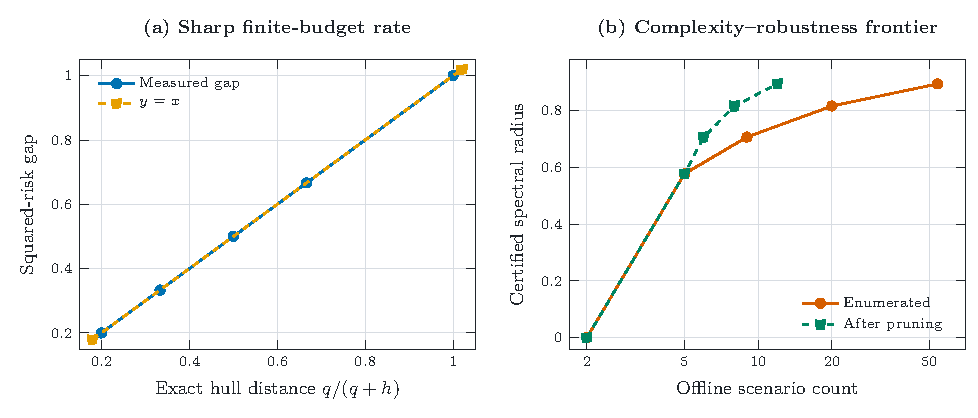
\includegraphics[width=\linewidth]{figures/budget_pareto.pdf}
  \caption{Finite hidden-budget hierarchy for the two-port fixed-rule audit
  $C=Q=2^{-1/2}[1\ \ 1]$.
  The measured finite-to-unbounded squared-risk gaps coincide numerically with
  the exact distance $q/(q+h)$.  Increasing the hidden budget increases both
  the certified radius and the offline scenario count; exact pruning deletes
  redundant LMIs without changing the radius.}
  \label{fig:budget-pareto}
\end{figure}

\section{Graph-smoothing examples and algorithmic meaning}

\subsection{A finite-budget gain that is not imposed by a protocol constraint}

Let $q=2$, $h=1$, and
$C=P_{\rm av}=\one\one^T/2$.  The five exact candidates are
\[
 \begin{gathered}
 I,\quad \diag(1/2,1),\quad \diag(1,1/2),\\
 P_{\rm av},\quad \tfrac23P_{\rm av}.
 \end{gathered}
\]
The unconstrained solution of \eqref{eq:finite-sdp} is
\begin{equation}
 Q_*=\tfrac23P_{\rm av},\qquad
 R_1^*=\tfrac{\sqrt2}{3}=0.471404\ldots .
 \label{eq:finite-example}
\end{equation}
At this $Q$, the scenario radii are
\[
 \tfrac13,\quad\tfrac{\sqrt7}{6},\quad\tfrac{\sqrt7}{6},
 \quad\tfrac13,\quad\tfrac{\sqrt2}{3}.
\]
The last scenario has the unavoidable hidden-input term
\[
 C\left(\frac23P_{\rm av}-\frac49P_{\rm av}\right)C^T
 =\frac29P_{\rm av},
\]
which proves optimality.  The unbounded optimum is $1/2$, so knowing $h=1$
reduces radius by $5.72\%$ and squared risk by $11.11\%$.  At $h=0$, the
choice $Q=C$ has zero error.

\subsection{Why unbounded design needs locality}

If $Q$ is unrestricted, $P=0$ and $P=I$ imply
\[
 \max_{P\in\cP_q^\partial}\norm{CP-Q}_2\geq\frac12\norm C_2,
\]
while $Q=C/2$ attains equality for every orthogonal projection $P$.  Thus the
unbounded free-$Q$ problem has the transparent solution
$Q_*=C/2$, $R_\infty^*=\norm C_2/2$.  Communication sparsity or another real
protocol restriction is required for a substantive design tradeoff.

For a minimal shared-opcode example, take
\[
 C=\diag(1,2),\qquad \cQ_{\rm loc}=\{\alpha I_2:\alpha\in\R\}.
\]
The exact five-scenario problem gives
\begin{equation}
\begin{aligned}
 \alpha_*&=\tfrac43-\tfrac{2\sqrt{10}}{15}
             =0.911696\ldots,\\
 R_*&=\tfrac{10+2\sqrt{10}}{15}
             =1.088304\ldots .
\end{aligned}
 \label{eq:shared-example}
\end{equation}
Dropping the connected partial scenario $P_{\rm av}$ instead gives the
incorrect answer $\alpha=1$, $R=1$: the robust radius is underestimated by
$8.83\%$.  This example also illustrates why the solver reports the active
scenario set rather than only the optimal matrix.

\subsection{Exact geometry versus a generic positive-contraction set}

The common surrogate $0\preceq X\preceq I$ is safe because it contains
$K_\infty$, but it need not be tight.  This difference is already analytic for
$q=2$, $d=1$, and the constant-preserving family
\begin{equation}
 C=[0\ \ 2],\qquad Q(a)=[a\ \ 2-a].
 \label{eq:outer-example-data}
\end{equation}
The exact five partial-partition scenarios give
\begin{equation}
\begin{aligned}
 R_{\rm exact}(a)=\max\{&[a^2+(2-a)^2]^{1/2},\\
                         &\sqrt2|a|,\ \sqrt2|1-a|\}.
\end{aligned}
\label{eq:exact-outer-comparison}
\end{equation}
Its optimum is $\sqrt2$ at $a=1$.  Maximizing the same affine Gram loss over
the full positive-contraction interval instead gives
\begin{equation}
 R_{[0,I]}(a)=1+\sqrt{a^2+(1-a)^2},
 \label{eq:outer-radius}
\end{equation}
whose optimum is $1+1/\sqrt2$ at $a=1/2$.  Exact terminal geometry therefore
lowers the optimal certified radius by $17.2\%$ in this example.  At the
network-optimal rule, the generic certificate is $2$ rather than $\sqrt2$, a
$41.4\%$ overestimate.  This example isolates geometric conservatism from
sampling failure and solver error.

\subsection{Offline and online costs}

Scenario generation, conic model construction, and SDP solution are offline
design costs.  They depend exponentially on the port boundary but not on the
eventual hidden network size.  Once $Q$ is fixed, online estimation is simply
$QE_\Gamma y$.  Under an $r$-hop zero pattern its operational accounting can
therefore be kept separate: $r$ synchronous rounds, protocol-dependent message
and byte-hop counts, $\operatorname{nnz}(Q)$ multiply-adds per signal, and
storage proportional to $\operatorname{nnz}(Q)$.  These quantities are not
part of the mathematical radius and should be reported separately in
experiments.

\begin{figure}[t]
  \centering
  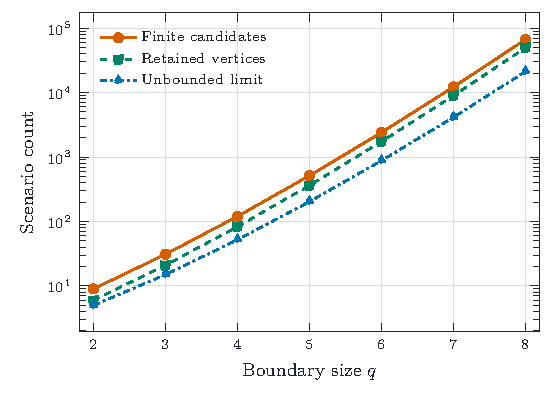
\includegraphics[width=0.76\linewidth]{figures/scenario_scaling.pdf}
  \caption{Exact scenario counts at hidden budget $h=2$.  Finite candidates,
  retained finite-hull vertices, and unbounded partial partitions all grow
  combinatorially with $q$.  The reduction is boundary-size fixed-parameter,
  not polynomial in the boundary size.}
  \label{fig:scenario-scaling}
\end{figure}

\section{Computational validation}

\subsection{Fixed theorem-matched design grid}

All main-paper experiments optimize the same full-input norm as the theorem.
The benchmark definition enumerates every cell before solving and reports all
of them: $q\in\{3,4,5\}$, $h\in\{1,2,4\}$, and six rule families per $q$,
for \CoreProblemCount{} exact design problems.  The six families are direct
state smoothing ($C=I$) with constant preservation $Q\one=\one$ at zero-hop,
one-hop, and full-port support on a fixed path overlay $H$; heterogeneous
diagonal outputs with independent or shared diagonal coefficients; and an
unconstrained one-hop state rule as a negative control.  For each cell, five
$N=32$ randomized designs use random-cyclic, grid, and geometric completions
with log-uniform weights in $[10^{-2},10^2]$ and hidden counts cycled through
$0,\ldots,h$, giving \CoreSamplingDesignCount{} sampled rules.  Every sampled
rule and every positive-contraction rule is evaluated afterward on the
complete exact finite scenario set.

Figure~\ref{fig:core-design} reports the two main comparisons.  Across the
nine matched $(q,h)$ state-smoothing pairs, one communication round reduces
the certified radius over zero-hop operation by a median
\OneHopMedianGainPct\%, while full-port support reduces it by
\FullPortMedianGainPct\% in the descriptive grid.  All nine one-hop solves
in the headline comparison have status \texttt{optimal}; the zero-hop
constraint fixes $Q=I$.  The unconstrained negative control is retained in
the archive: without constant preservation, the robust center can collapse to
a diagonal/no-communication rule, so communication is not beneficial by
construction.  Over the one-hop constant-preserving subgroup, the generic
$0\preceq X\preceq I$ design has median exact-risk overhead
\OneHopPSDMedianOverheadPct\%; over the full grid it is often tight, which is
why the complete distribution rather than only favorable cases is shown.

\begin{figure*}[t]
  \centering
  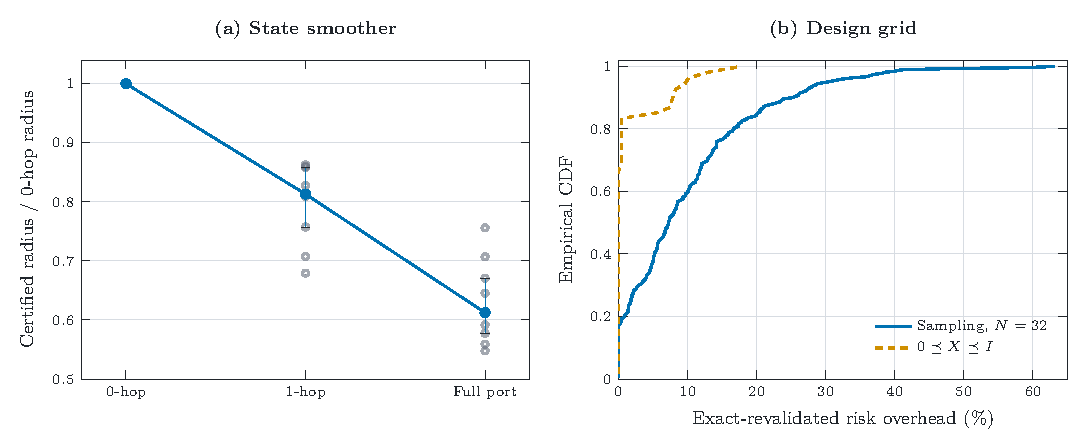
\includegraphics[width=\textwidth]{figures/core_design_benchmark.pdf}
  \caption{Fixed theorem-matched design grid.  (a) Postsolve-revalidated
  radii for nine $(q,h)$ pairs under three support classes (27 evaluations),
  normalized by the corresponding zero-hop radius; gray circles show all
  pairs and blue markers show median and interquartile range.  (b) Descriptive
  empirical CDFs of exact-revalidated true-risk overhead for 270 $N=32$
  sampled rules and 54 finite-budget evaluations of 18 positive-contraction
  designs.  These grouped grid evaluations are not treated as IID samples.}
  \label{fig:core-design}
\end{figure*}

The representative state problem has $q=4$, $h=1$, $C=I$, one-hop path
support, and $Q\one=\one$.  Its deployed exact rule is
\begin{equation}
 Q_*\!=\!\begin{bmatrix}
 .726&.274&0&0\\ .094&.630&.276&0\\
 0&.276&.630&.094\\ 0&0&.274&.726
 \end{bmatrix},
 \label{eq:principal-rule}
\end{equation}
with exact radius \PrincipalExactRadius.  The unbounded optimum is
\PrincipalUnboundedRadius, so using the known one-node hidden budget improves
the radius by \PrincipalFiniteGainPct\%.  The positive-contraction design has
exact finite risk \PrincipalPSDTrueRadius, or \PrincipalPSDOverheadPct\%
overhead after exact reevaluation.  Thresholding solver-scale entries at
$2\times10^{-5}$ and recertifying gives an implementation with
\PrincipalRounds{} round, \PrincipalScalarHops{} scalar-hops
(48 byte-hops in double precision), \PrincipalOnlineFlops{} online FLOPs, and
\PrincipalStorageBytes{} bytes of sparse coefficient storage.  These are
counts for one explicit unicast schedule, not communication lower bounds.

\subsection{Sampling budget and physical path tightness}

To avoid a train--test distribution shift, the sampling study draws nested
training sets from the same distribution at
$N\in\{4,8,16,32,64,128,256\}$.  It uses 30 independent seeds for the
four-port state problem above and for a three-port, two-hidden-node shared
diagonal-opcode problem.  Thus there are \SamplingCurveRunCount{} fitted
rules.  For a sampled rule $Q_N$, let $R_N(Q_N)$ be its maximum training
radius, $R_h(Q_N)$ its exact finite-budget radius, and $R_h^*$ the robust
optimum.  We report relative underreporting
$[R_h(Q_N)-R_N(Q_N)]/R_h(Q_N)$ and regret $R_h(Q_N)/R_h^*-1$; a failure means
$R_h(Q_N)-R_N(Q_N)>\max\{2\times10^{-5},10^{-3}R_h(Q_N)\}$.  At every sample
size and in both cases, all 30 rules fail this test; the per-cell 95\% Wilson
lower bound on this descriptive failure frequency is \SamplingWilsonLowPct\%.
At $N=32$,
the state problem has median underreporting
\PrincipalSampleUnderMedianPct\% and median true-risk regret
\PrincipalSampleRegretMedianPct\%.  Figure~\ref{fig:sampling-budget} shows that
both gaps have an overall downward trend with $N$ but remain nonzero at 256;
sampling is therefore a useful design heuristic, not a deterministic
certificate.

\begin{figure*}[t]
  \centering
  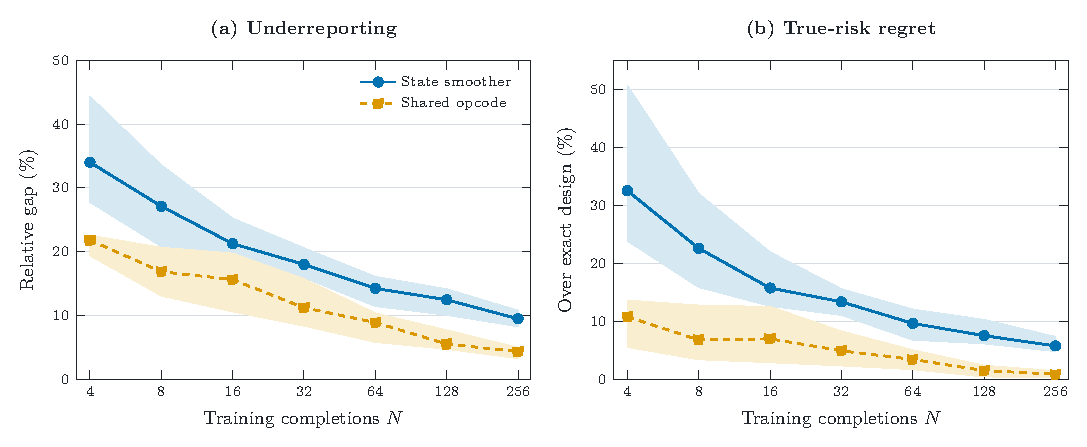
\includegraphics[width=\textwidth]{figures/sampling_budget_curve.pdf}
  \caption{Same-distribution randomized design with 30 seeds per point; bands
  are interquartile ranges.  (a) Relative gap between exact-revalidated and
  training radii.  (b) Exact-revalidated risk overhead over exact robust
  design.  Training samples are nested within each seed.}
  \label{fig:sampling-budget}
\end{figure*}

Finally, we instantiate the converse rather than checking only algebraic
scenarios.  Three active finite vertices with one, two, and three partition
blocks are realized by connected paths containing exactly $h=1$ hidden node.
Within-component conductance is $t$, bridge conductance is $t^{-1}$, and
$t$ ranges from $10$ to $10^6$.  At the final value, the largest relative
full-input risk gap is $\PathMaxFinalRiskGap$ and the largest port-block
operator gap is $\PathMaxFinalBlockGap$; every constructed graph is connected
and has maximum degree two.  Figure~\ref{fig:path-tightness} makes the physical
attainability behind the lower-bound proof numerically visible.

\begin{figure*}[t]
  \centering
  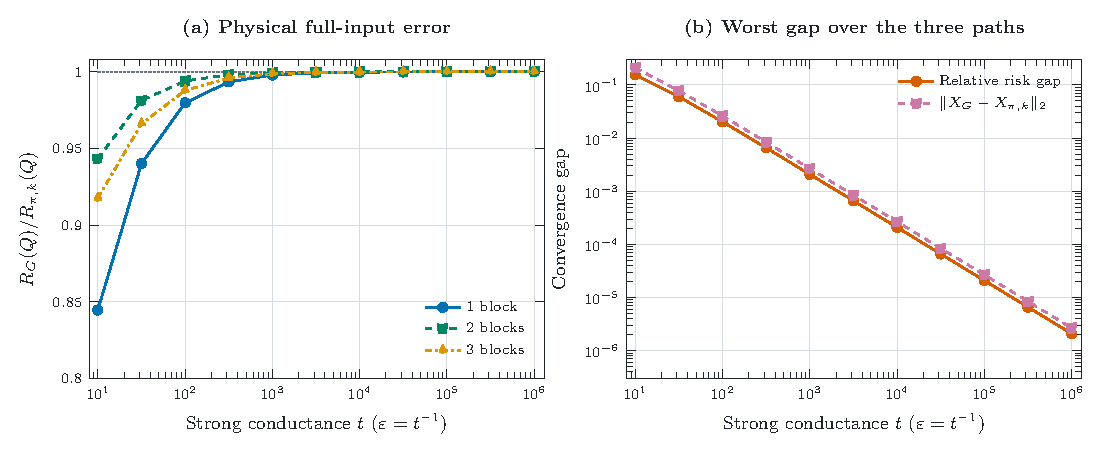
\includegraphics[width=\textwidth]{figures/path_tightness.pdf}
  \caption{Connected maximum-degree-two path witnesses for three active exact
  scenarios.  (a) Physical full-input risk approaches its canonical value.
  (b) Both the worst relative risk gap and port-block operator distance vanish
  as strong and weak conductances separate.}
  \label{fig:path-tightness}
\end{figure*}

As implementation audits, a separate 135-completion sweep places every sampled
physical error below its exact certificate (largest ratio $0.9475$), and the
pruned and unpruned smoke-test radii agree to $1.7\times10^{-9}$.  At $q=8$,
$h=2$, generation yields 66,491 candidates, 49,484 retained vertices, and
21,147 partial partitions, exposing the intended boundary-size limit.
On the archived platform, all \CoreProblemCount{} finite designs completed in
median \CoreExactMedianTotalSeconds{} s and maximum
\CoreExactMaxTotalSeconds{} s end to end; the slowest cell had
$q=\CoreExactMaxQ$, $h=\CoreExactMaxH$.  These one-pass timings are descriptive.
Fixed-known-graph local algorithms, PGLib/SuiteSparse scale tests
\cite{babaeinejadsarookolaee2019pglib,davis2011suitesparse}, and accelerator
timings are reported separately in the supplement because they test a
different known-topology task or a particular hardware implementation.

The archived solver accepts $C$, $q$, $h$ (or unbounded mode), and affine local
rules, and returns $Q$, its exact-revalidated radius, active scenarios, counts,
and timings.  The anonymous software supplement contains fixed configurations,
records, seeds, provenance, tests, figure sources, and reproduction commands;
a permanent repository can replace it after review.

\section{Discussion and Scope Boundaries}

The following boundaries are part of the result rather than optional
qualifications.

\begin{itemize}[leftmargin=1.5em]
\item Finite-$h$ equality assumes scalar undirected nonnegative edges and unit
grounding.  A uniform finite upper bound on conductance can destroy the
high-conductance converse, and a positive lower bound on connecting edges can
destroy weak-link separation.
\item Hidden-input columns cannot be discarded.  For finite scenarios they
produce $C(X-X^2)C^T$ in \eqref{eq:gram-identity}.
\item The protocol overlay $H$ is fixed independently of the physical
completion $G$.  If communication edges must instead be inferred from $G$,
the admissible rule class varies with the uncertainty and is a different
problem.
\item The unbounded partial-partition reduction for full errors is sharp at
Schatten exponent two.  It is not a theorem for arbitrary convex losses of the
full error matrix, and it fails for every Schatten exponent below two.
\item The estimator in \eqref{eq:smoother} is graph-regularized state
smoothing.  A raw WLS measurement-noise transfer includes the measurement
operator as an additional right factor; its MSE is not
$\norm{\cA_G(Q)}_F^2$ without a separate derivation.
\item The theorem does not cover directed, signed, block-noncommutative, or
nonlinear completion models.
\end{itemize}

The exact method is most attractive when an arbitrarily large hidden network
attaches to a modest port boundary.  Bell-number growth in $q$ eventually
dominates offline design, as Figure~\ref{fig:scenario-scaling} shows; scalable
separation, cutting-plane, and symmetry reductions remain outside the present
claims.

\section{Conclusion}

Unknown hidden topology need not be sampled or replaced by a full-block
uncertainty set for this graph smoother.  Set partitions and hidden-budget
allocations give an exact finite description, including the complete hidden
input, while connected paths certify that every retained boundary scenario is
genuinely sharp.  The result supplies a lossless SDP for constrained common
local rules and an exact budget-to-unbounded convergence rate.  The numerical
results separate exact certification from completion sampling and generic
positive-contraction relaxation; fixed-graph approximation remains a different
task.

\bibliographystyle{IEEEtran}
\begingroup
\sloppy
\bibliography{references}
\endgroup

\end{document}
